\documentclass[aspectratio=169,11pt]{beamer}

% Theme and colors
\usetheme{Madrid}
\usecolortheme{whale}
\setbeamertemplate{navigation symbols}{}
\setbeamertemplate{footline}{\hfill\insertframenumber}

% Packages
\usepackage[utf8]{inputenc}
\usepackage[T1]{fontenc}
\usepackage{amsmath,amssymb,amsfonts}
\usepackage{graphicx}
\usepackage{booktabs}
\usepackage{tikz}
\usepackage{algorithm2e}
\usepackage{listings}
\usepackage{hyperref}
\usepackage{xcolor}
\usepackage{multirow}
\usepackage{adjustbox}

% Custom colors
\definecolor{dauphine}{RGB}{0,62,107}
\definecolor{highlight}{RGB}{220,50,47}
\definecolor{codegreen}{RGB}{0,128,0}

\setbeamercolor{title}{fg=white,bg=dauphine}
\setbeamercolor{frametitle}{fg=white,bg=dauphine}
\setbeamercolor{block title}{fg=white,bg=dauphine}

% Code listing style
\lstset{
    basicstyle=\tiny\ttfamily,
    keywordstyle=\color{blue},
    commentstyle=\color{codegreen},
    stringstyle=\color{red},
    numbers=left,
    numberstyle=\tiny,
    frame=single,
    breaklines=true
}

% Title information
\title[Time-Varying Factor Allocation]{\textbf{Replication: Time-Varying Factor Allocation}}
\subtitle{Vincenz \& Zeissler (2022)}
\author{Thomas BETTON, Pierre BERTHOLD, Chadi RAIS, Pierre LIBERGE}
\institute{Universit\'e Paris-Dauphine\\Master Gestion Quantitative}
\date{\today}

\begin{document}

% =============================================================================
% TITLE
% =============================================================================
\begin{frame}
    \titlepage
\end{frame}

% =============================================================================
% TABLE OF CONTENTS
% =============================================================================
\begin{frame}{Plan de la Pr\'esentation}
    \begin{enumerate}
        \item Introduction et Motivation
        \item Donn\'ees et Sources
        \item Construction des Facteurs
        \item Variables Pr\'edictives
        \item R\'egression Bay\'esienne Pr\'edictive
        \item Allocation Black-Litterman
        \item R\'esultats
        \item Diff\'erences avec le Papier
        \item Calibration et Sensibilit\'e
        \item Conclusion
        \item Extensions
    \end{enumerate}
\end{frame}

% =============================================================================
% SECTION 1: INTRODUCTION
% =============================================================================
\section{Introduction et Motivation}

\begin{frame}{Contexte et Objectifs}
    \begin{block}{Article de R\'ef\'erence}
        \textbf{``Time-Varying Factor Allocation''} -- Vincenz \& Zeissler (2022)
        \begin{itemize}
            \item Publi\'e dans \textit{The Journal of Portfolio Management}
            \item P\'eriode d'\'etude: 1973--2018 (45 ans)
        \end{itemize}
    \end{block}

    \vspace{0.3cm}

    \begin{block}{Question Centrale}
        \textit{Peut-on am\'eliorer la performance d'un portefeuille multi-facteurs en utilisant des pr\'edicteurs macro\'economiques et de march\'e?}
    \end{block}

    \vspace{0.3cm}

    \begin{alertblock}{Contribution Principale}
        Combinaison de:
        \begin{enumerate}
            \item R\'egression bay\'esienne pr\'edictive (pr\'evisions conservatrices)
            \item Allocation Black-Litterman (gestion du risque actif)
        \end{enumerate}
    \end{alertblock}
\end{frame}

\begin{frame}{Architecture G\'en\'erale de la Strat\'egie}
    \begin{center}
    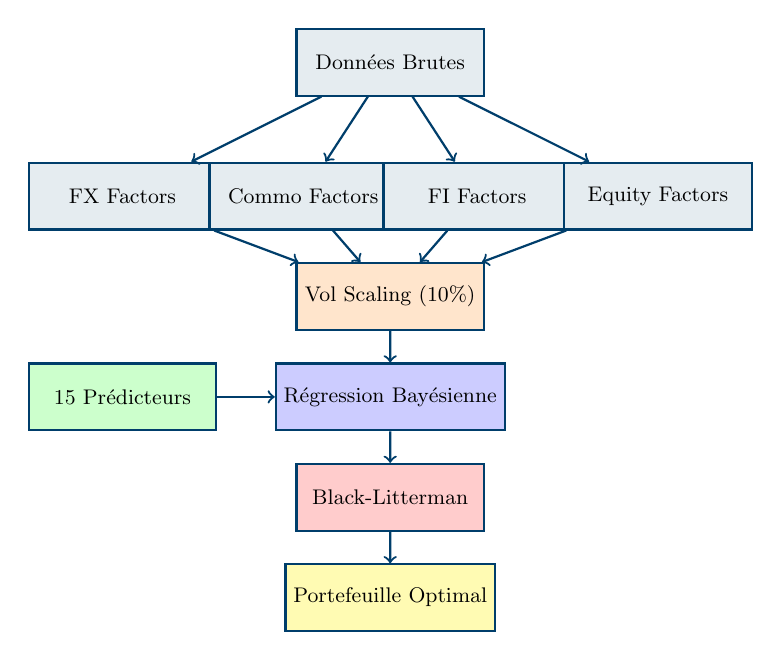
\begin{tikzpicture}[scale=0.85, transform shape,
        box/.style={rectangle, draw=dauphine, fill=dauphine!10, thick, minimum height=1cm, minimum width=2.8cm, text centered, font=\small},
        arrow/.style={->, thick, dauphine}]

        % Data layer
        \node[box] (data) at (0,4) {Donn\'ees Brutes};

        % Factor layer
        \node[box] (fx) at (-4,2) {FX Factors};
        \node[box] (commo) at (-1.3,2) {Commo Factors};
        \node[box] (fi) at (1.3,2) {FI Factors};
        \node[box] (eq) at (4,2) {Equity Factors};

        % Volatility scaling
        \node[box, fill=orange!20] (volscale) at (0,0.5) {Vol Scaling (10\%)};

        % Predictors
        \node[box, fill=green!20] (pred) at (-4,-1) {15 Pr\'edicteurs};

        % Bayesian
        \node[box, fill=blue!20] (bayes) at (0,-1) {R\'egression Bay\'esienne};

        % Black-Litterman
        \node[box, fill=red!20] (bl) at (0,-2.5) {Black-Litterman};

        % Output
        \node[box, fill=yellow!30] (port) at (0,-4) {Portefeuille Optimal};

        % Arrows
        \draw[arrow] (data) -- (fx);
        \draw[arrow] (data) -- (commo);
        \draw[arrow] (data) -- (fi);
        \draw[arrow] (data) -- (eq);

        \draw[arrow] (fx) -- (volscale);
        \draw[arrow] (commo) -- (volscale);
        \draw[arrow] (fi) -- (volscale);
        \draw[arrow] (eq) -- (volscale);

        \draw[arrow] (volscale) -- (bayes);
        \draw[arrow] (pred) -- (bayes);
        \draw[arrow] (bayes) -- (bl);
        \draw[arrow] (bl) -- (port);

    \end{tikzpicture}
    \end{center}
\end{frame}

% =============================================================================
% SECTION 2: DATA
% =============================================================================
\section{Donn\'ees et Sources}

\begin{frame}{Sources de Donn\'ees}
    \begin{columns}[T]
        \begin{column}{0.5\textwidth}
            \begin{block}{Classes d'Actifs}
                \begin{itemize}
                    \item \textbf{Devises (FX)}: 59 paires vs USD
                        \begin{itemize}
                            \item GBP, EUR, JPY, CHF, CAD, AUD, NZD, SEK, NOK...
                        \end{itemize}
                    \item \textbf{Commodities}: Futures front \& 2nd month
                        \begin{itemize}
                            \item Energie, M\'etaux, Agriculture
                        \end{itemize}
                    \item \textbf{Taux (FI)}: Rendements souverains
                        \begin{itemize}
                            \item 10Y yields multi-pays
                        \end{itemize}
                    \item \textbf{Actions (Equity)}: Indices MSCI
                \end{itemize}
            \end{block}
        \end{column}
        \begin{column}{0.5\textwidth}
            \begin{block}{Variables Pr\'edictives}
                \begin{itemize}
                    \item \textbf{Macro US}:
                        \begin{itemize}
                            \item CFNAI, CPI YoY, 3M T-Bill
                            \item Yield Curve (10Y-2Y)
                        \end{itemize}
                    \item \textbf{March\'e}:
                        \begin{itemize}
                            \item VIX, SKEW, TED Spread
                        \end{itemize}
                    \item \textbf{Global}:
                        \begin{itemize}
                            \item Budget Balance, M2 Growth
                        \end{itemize}
                \end{itemize}
            \end{block}

            \begin{alertblock}{Source}
                Bloomberg via DataGestionQuant.xlsx
            \end{alertblock}
        \end{column}
    \end{columns}
\end{frame}

\begin{frame}{Traitement des Donn\'ees}
    \begin{block}{Nettoyage et Pr\'eparation}
        \begin{enumerate}
            \item \textbf{Filtrage}: Minimum 120 observations valides par s\'erie
            \item \textbf{Outliers}: Clipping des rendements extr\^emes
                \begin{itemize}
                    \item FX: $[-30\%, +30\%]$
                    \item Commodities: $[-50\%, +50\%]$
                    \item Fixed Income: $[-20\%, +20\%]$
                \end{itemize}
            \item \textbf{Alignement}: Resampling mensuel (fin de mois)
        \end{enumerate}
    \end{block}

    \begin{block}{Calcul des Rendements}
        \begin{itemize}
            \item \textbf{FX}: Rendements spot + diff\'erentiel de taux (excess returns)
            \item \textbf{Commodities}: Rendements du contrat front month
            \item \textbf{Fixed Income}: $r_t \approx \frac{y_{t-1}}{12} - D \cdot \Delta y_t$ (duration $D=7$)
            \item \textbf{Equity}: Rendements total return index
        \end{itemize}
    \end{block}
\end{frame}

% =============================================================================
% SECTION 3: FACTOR CONSTRUCTION
% =============================================================================
\section{Construction des Facteurs}

\begin{frame}{Portefeuilles Long-Short: M\'ethodologie (1/2)}
    \begin{block}{Tri en Sextiles}
        Pour chaque signal $s_{i,t}$ (carry, momentum, value):
        \begin{enumerate}
            \item Classer les actifs par signal
            \item Diviser en 6 groupes (sextiles)
            \item \textbf{Long}: Top 16.67\% (meilleur sextile)
            \item \textbf{Short}: Bottom 16.67\% (pire sextile)
        \end{enumerate}
    \end{block}
\end{frame}

\begin{frame}{Portefeuilles Long-Short: M\'ethodologie (2/2)}
    \begin{block}{Poids du Portefeuille}
        $$w_{i,t} = \begin{cases}
            +\frac{1}{n_{top}} & \text{si } rank(s_{i,t}) > N - \frac{N}{6} \\[5pt]
            -\frac{1}{n_{bottom}} & \text{si } rank(s_{i,t}) \leq \frac{N}{6} \\[5pt]
            0 & \text{sinon}
        \end{cases}$$
    \end{block}

    \begin{alertblock}{Rendement du Facteur}
        $r_{factor,t} = \sum_{i} w_{i,t-1} \cdot r_{i,t}$ \quad (poids d\'ecal\'es d'un mois)
    \end{alertblock}
\end{frame}


\begin{frame}{Facteurs FX (4 facteurs)}
    \begin{block}{FX Market}
        Rendement moyen \'equi-pond\'er\'e de toutes les devises vs USD
        $$r_{FX.Mkt,t} = \frac{1}{N}\sum_{i=1}^{N} r^{excess}_{i,t}$$
    \end{block}

    \begin{block}{FX Carry}
        Signal = Diff\'erentiel de taux d'int\'er\^et
        $$s^{carry}_{i,t} = r^{foreign}_i - r^{USD}$$
        Long devises \`a taux \'elev\'e, short devises \`a taux faible
    \end{block}

    \begin{block}{FX Momentum (12-1)}
        Signal = Rendement cumul\'e sur 12 mois (excluant le dernier)
        $$s^{mom}_{i,t} = \prod_{k=2}^{12}(1 + r_{i,t-k}) - 1$$
    \end{block}
\end{frame}

\begin{frame}{Facteurs FX -- Value (1/2)}
    \begin{block}{D\'efinition du Papier}
        \textbf{Value} = Variation sur 5 ans du taux de change r\'eel
        $$s^{value}_{i,t} = \Delta_{5y}\left(s_i - p_{US} + p_i^*\right)$$
        o\`u $s$ = spot, $p$ = indice des prix (CPI)
    \end{block}
\end{frame}

\begin{frame}{Facteurs FX -- Value (2/2)}
    \begin{alertblock}{Notre Approximation}
        \textbf{Limitation}: Pas de donn\'ees CPI par pays disponibles

        \vspace{0.2cm}

        \textbf{Proxy utilis\'e}: D\'eviation par rapport \`a la moyenne mobile 5 ans
        $$s^{value}_{i,t} = -\left(\frac{P_{i,t}}{MA_{60}(P_i)} - 1\right)$$

        \begin{itemize}
            \item N\'egatif = devise ``ch\`ere'' $\rightarrow$ Short
            \item Positif = devise ``bon march\'e'' $\rightarrow$ Long
        \end{itemize}
    \end{alertblock}
\end{frame}


\begin{frame}{Facteurs Commodities (5 facteurs)}
    \begin{columns}[T]
        \begin{column}{0.5\textwidth}
            \begin{block}{Market}
                $$r_{Commo.Mkt,t} = \frac{1}{N}\sum_{i} r_{i,t}$$
            \end{block}

            \begin{block}{Carry (Roll Yield)}
                \textbf{Papier}: $s^{carry} = \frac{F^{T2}}{F^{T1}} - 1$
                \begin{itemize}
                    \item Contango (+) $\rightarrow$ Short
                    \item Backwardation (-) $\rightarrow$ Long
                \end{itemize}
                Signal invers\'e avant ranking
            \end{block}

            \begin{block}{Momentum (12-1)}
                Comme pour FX
            \end{block}
        \end{column}
        \begin{column}{0.5\textwidth}
            \begin{block}{Value}
                \textbf{Papier}: $s^{value} = -\sum_{k=1}^{60} r_{t-k}$

                Rendement cumul\'e 5 ans n\'egatif

                \vspace{0.2cm}

                \textbf{Impl\'ementation}:
                $$s^{value}_{i,t} = -\left(\frac{P_{i,t}}{P_{i,t-60}} - 1\right)$$
            \end{block}

            \begin{block}{Basis-Momentum}
                Variation du roll yield sur 12 mois
                $$s^{bm}_{i,t} = \Delta_{12}\left(\frac{F^{T2}}{F^{T1}}\right)$$
            \end{block}
        \end{column}
    \end{columns}
\end{frame}

\begin{frame}{Facteurs Fixed Income (4 facteurs)}
    \begin{block}{Calcul des Rendements Obligataires}
        Approximation via duration:
        $$r_{bond,t} \approx \frac{y_{t-1}}{12} - D \cdot \Delta y_t$$
        avec Duration $D = 7$ ans pour obligations 10Y
    \end{block}

    \begin{columns}[T]
        \begin{column}{0.5\textwidth}
            \begin{block}{FI Carry}
                \textbf{Papier}: Pente de la courbe
                $$s^{carry} = y^{10Y} - y^{5Y}$$

                \textbf{Impl\'ementation}:
                \begin{itemize}
                    \item Utilise 10Y-5Y si disponible
                    \item Fallback: niveau du yield 10Y
                \end{itemize}
            \end{block}
        \end{column}
        \begin{column}{0.5\textwidth}
            \begin{block}{FI Value and FI Momentum}
                Yield relatif \`a sa moyenne historique
                $$s^{value} = \frac{y_t}{MA_{60}(y)} - 1$$
                Yield \'elev\'e vs historique = ``cheap''
                Momentum : Rendement cumul\'e 12-1 mois
            \end{block}

        \end{column}
    \end{columns}
\end{frame}

\begin{frame}{Facteurs Equity (4 facteurs)}
    \begin{block}{Universe}
        Indices MSCI par pays (utilisation des Total Return Indices)
    \end{block}

    \begin{columns}[T]
        \begin{column}{0.5\textwidth}
            \begin{block}{Equity Market}
                Rendement moyen \'equi-pond\'er\'e
            \end{block}

            \begin{block}{Equity Momentum}
                Signal 12-1 mois standard
            \end{block}
        \end{column}
        \begin{column}{0.5\textwidth}
            \begin{block}{Equity Size}
                Signal = $-\log(MarketCap)$

                Long small caps, short large caps
            \end{block}

            \begin{block}{Equity Value}
                Proxy: Prix vs MA 5 ans
                $$s^{value} = \frac{MA_{60}(P)}{P} - 1$$
            \end{block}
        \end{column}
    \end{columns}

    \begin{alertblock}{Note}
        Le papier utilise 21 facteurs; notre impl\'ementation en a \textbf{17} du fait de limitations de donn\'ees (pas de facteurs Quality, Low-Vol, etc.)
    \end{alertblock}
\end{frame}

\begin{frame}{Volatility Scaling}
    \begin{block}{Objectif}
        Normaliser tous les facteurs et permet de comparer les facteurs sur une base de risque \'equivalente \`a \textbf{10\% de volatilit\'e annualis\'ee ex-ante}
    \end{block}

    \begin{block}{M\'ethodologie}
        \begin{enumerate}
            \item Calculer la volatilit\'e rolling (36 mois, minimum 12)
            $$\sigma_{t} = \text{std}(r_{t-36:t}) \times \sqrt{12}$$

            \item Appliquer le facteur d'\'echelle
            $$\text{scale}_t = \frac{0.10}{\sigma_{t-1}}$$

            \item Clipper le levier: $\text{scale} \in [0.1, 3.0]$

            \item Rendements ajust\'es
            $$r^{scaled}_t = r_t \times \text{scale}_t$$
        \end{enumerate}
    \end{block}
\end{frame}

% =============================================================================
% SECTION 4: PREDICTORS
% =============================================================================
\section{Variables Pr\'edictives}

\begin{frame}{Les 15 Pr\'edicteurs du Papier}
    \begin{columns}[T]
        \begin{column}{0.5\textwidth}
            \begin{block}{Signaux Macro\'economiques}
                \begin{enumerate}
                    \item \textbf{CFNAI}: Chicago Fed Activity Index
                    \item \textbf{Inflation}: CPI YoY
                    \item \textbf{Short Rate}: Taux 3M US
                    \item \textbf{Yield Curve}: 10Y - 2Y
                    \item \textbf{Budget Balance}: Balance fiscale mondiale
                    \item \textbf{M2 Growth}: Croissance masse mon\'etaire
                \end{enumerate}
            \end{block}
        \end{column}
        \begin{column}{0.5\textwidth}
            \begin{block}{Signaux de March\'e}
                \begin{enumerate}
                    \setcounter{enumi}{6}
                    \item \textbf{VIX}: Volatilit\'e implicite
                    \item \textbf{TED Spread}: Stress cr\'edit
                    \item \textbf{SKEW}: Risque de queue
                    \item \textbf{EPU}: Incertitude politique
                \end{enumerate}
            \end{block}

            \begin{block}{Signaux Factoriels}
                \begin{enumerate}
                    \setcounter{enumi}{10}
                    \item \textbf{TS-Mom}: Momentum 12M facteurs
                    \item \textbf{TS-Vol}: Volatilit\'e 12M facteurs
                \end{enumerate}
            \end{block}
        \end{column}
    \end{columns}

    \vspace{0.3cm}

    \begin{alertblock}{Pr\'edicteurs Manquants}
        RTS.10Y, TS-Value, FCTR.SPRD non impl\'ement\'es (donn\'ees manquantes)
    \end{alertblock}
\end{frame}

\begin{frame}{Standardisation des Pr\'edicteurs}
    \begin{block}{M\'ethode Expanding Window}
        Pour \'eviter le look-ahead bias:
        $$z_{t} = \frac{x_t - \mu_{1:t}}{\sigma_{1:t}}$$

        \begin{itemize}
            \item $\mu_{1:t}$ = moyenne de toutes les observations jusqu'\`a $t$
            \item $\sigma_{1:t}$ = \'ecart-type de toutes les observations jusqu'\`a $t$
            \item Minimum 120 observations avant de commencer
        \end{itemize}
    \end{block}

    \begin{block}{Cas Sp\'eciaux}
        \begin{itemize}
            \item \textbf{TED Spread}: Donn\'ees Bloomberg invalides $\rightarrow$ proxy HY Spread
            \item \textbf{Budget Balance}: S\'erie courte (2001-2017) $\rightarrow$ lookback 36 mois
            \item \textbf{M2 Growth}: Utilise le taux de croissance YoY, pas le niveau
        \end{itemize}
    \end{block}
\end{frame}

% =============================================================================
% SECTION 5: BAYESIAN REGRESSION
% =============================================================================
\section{R\'egression Bay\'esienne Pr\'edictive}

\begin{frame}{Mod\`ele de Pr\'ediction}
    \begin{block}{R\'egression Lin\'eaire}
        Pour chaque paire (facteur $f$, pr\'edicteur $x$):
        $$r_{f,t+1} = \alpha + \beta \cdot x_t + \varepsilon_t$$
    \end{block}

    \begin{block}{Probl\`eme}
        OLS standard surestime la pr\'edictabilit\'e:
        \begin{itemize}
            \item $R^2$ in-sample souvent $> 5\%$
            \item Performance out-of-sample bien plus faible
            \item Risque de sur-apprentissage
        \end{itemize}
    \end{block}

    \begin{alertblock}{Solution Bay\'esienne}
        Utiliser un \textbf{prior conservateur} qui ``shrink'' les coefficients vers z\'ero

        $\rightarrow$ Implicitement: $R^2 < 1\%$ a priori
    \end{alertblock}
\end{frame}

\begin{frame}{Framework Bay\'esien}
    \begin{block}{Prior sur $\beta$}
        $$\beta \sim \mathcal{N}(0, \sigma^2_\eta)$$

        o\`u $\sigma^2_\eta = R^2_{prior} \cdot \frac{\text{Var}(y)}{\text{Var}(x)}$

        \vspace{0.2cm}

        Avec $R^2_{prior} = 0.01$ (1\%)
    \end{block}

    \begin{block}{Posterior}
        $$\beta_{Bayes} = \frac{\text{precision}_{OLS}}{\text{precision}_{OLS} + \text{precision}_{prior}} \cdot \beta_{OLS}$$

        \begin{itemize}
            \item $\text{precision}_{OLS} = \frac{\sum x^2}{\sigma^2_\varepsilon}$
            \item $\text{precision}_{prior} = \frac{1}{\sigma^2_\eta}$

        Avec prior $R^2 = 1\%$, les pr\'edictions sont tr\`es conservatrices
        \end{itemize}
    \end{block}
\end{frame}

\begin{frame}{Impl\'ementation Expanding Window}
    \begin{block}{Proc\'edure (pour chaque mois $t$)}
        \begin{enumerate}
            \item Utiliser les donn\'ees $\{1, ..., t\}$ pour estimer $\alpha$, $\beta$
            \item Appliquer le shrinkage bay\'esien
            \item Pr\'edire $\hat{r}_{t+1} = \alpha + \beta_{Bayes} \cdot x_t$
        \end{enumerate}
    \end{block}

    \begin{alertblock}{Output}
        Matrice de pr\'edictions: $\hat{R} \in \mathbb{R}^{T \times N_{facteurs}}$ pour chaque pr\'edicteur
    \end{alertblock}
\end{frame}

% =============================================================================
% SECTION 6: BLACK-LITTERMAN
% =============================================================================
\section{Allocation Black-Litterman}

\begin{frame}{Framework Black-Litterman}
    \begin{block}{Benchmark}
        Portefeuille \'equi-pond\'er\'e sur les $N$ facteurs
        $$w_{bench} = \frac{1}{N} \cdot \mathbf{1}$$
    \end{block}

    \begin{block}{Views}
        Les pr\'edictions bay\'esiennes fournissent les ``views'' sur les rendements futurs
        $$\hat{r}_{t+1} = \text{prediction from Bayesian regression}$$
    \end{block}

    \begin{block}{Objectif}
        Maximiser l'utilit\'e mean-variance avec tracking error:
        $$\max_w \quad \mathbb{E}[\alpha] - \frac{\lambda}{2} \cdot \text{Var}[\alpha]$$

        o\`u $\alpha = (w - w_{bench})' \cdot r$ est le rendement actif
    \end{block}
\end{frame}

\begin{frame}{Optimisation sous Contraintes}
    \begin{block}{Programme d'Optimisation}
        \begin{align*}
            \max_w \quad & (w - w_{bench})' \cdot \hat{r} - \frac{\lambda}{2}(w - w_{bench})' \Sigma (w - w_{bench})\\
            \text{s.t.} \quad & \sum_i w_i = 1 \quad \text{(fully invested)}\\
            & w_i \geq 0 \quad \forall i \quad \text{(long-only)}\\
            & w_i \leq 0.30 \quad \forall i \quad \text{(concentration limit)}
        \end{align*}
    \end{block}

    \begin{block}{Param\`etres}
        \begin{itemize}
            \item $\lambda = 5.0$ (aversion au risque de tracking error)
            \item Covariance $\Sigma$ estim\'ee sur 60 mois rolling
            \item Confiance dans les views: 50\% $\times$ scale par pr\'edicteur
            \item Tracking Error moyen $\approx 2-3\%$ (cible du papier)
        \end{itemize}
    \end{block}

\end{frame}

\begin{frame}{Gestion du Tracking Error}
    \begin{block}{Approche du Papier}
        Le TE n'est \textbf{pas} une contrainte dure mais un terme de p\'enalit\'e:
        $$\text{TE}^2 = (w - w_{bench})' \Sigma (w - w_{bench})$$
    \end{block}

    \begin{block}{Comportement}
        \begin{itemize}
            \item Signal fort $\rightarrow$ positions actives plus grandes $\rightarrow$ TE plus \'elev\'e
            \item Signal faible $\rightarrow$ proche du benchmark $\rightarrow$ TE faible
            \item Moyenne long-terme $\approx 2\%$ annualis\'e
        \end{itemize}
    \end{block}

    \begin{block}{Co\^uts de Transaction}
        Appliqu\'es ex-post: 10 bps one-way sur le turnover
        $$r_{net,t} = r_{gross,t} - TC \times \sum_i |w_{i,t} - w_{i,t-1}|$$
    \end{block}
\end{frame}

% =============================================================================
% SECTION 7: RESULTS
% =============================================================================
\section{R\'esultats}

\begin{frame}{Performance Cumul\'ee}
    \begin{center}
        \includegraphics[width=0.85\textwidth]{fig1_cumulative_returns.png}
    \end{center}
\end{frame}

\begin{frame}{Information Ratios par Strat\'egie}
    \begin{center}
        \includegraphics[width=0.9\textwidth]{fig2b_information_ratios_horizontal.png}
    \end{center}

    \begin{block}{Interpr\'etation}
        \begin{itemize}
            \item IR $> 0.5$: Excellent pour une strat\'egie de timing
            \item Meilleurs pr\'edicteurs: ShortRate, CFNAI, Inflation
            \item Coh\'erent avec les r\'esultats du papier
        \end{itemize}
    \end{block}
\end{frame}

\begin{frame}{Analyse par Sous-P\'eriodes}
    \begin{center}
        \includegraphics[width=0.85\textwidth]{fig4_subperiod_analysis.png}
    \end{center}

    \begin{block}{Observations}
        Persistance des meilleurs pr\'edicteurs \`a travers diff\'erentes p\'eriodes
    \end{block}
\end{frame}

\begin{frame}{Analyse des Drawdowns}
    \begin{center}
        \includegraphics[width=0.85\textwidth]{fig6_drawdowns.png}
    \end{center}
\end{frame}

\begin{frame}{R\'esum\'e Statistique}
    \begin{block}{Tests de Significativit\'e}
        \begin{itemize}
            \item Test t $> 1.96$ pour significativit\'e \`a 5\%
            \item Correction de Holm-Bonferroni pour tests multiples
        \end{itemize}
    \end{block}

    \begin{table}[h]
        \centering
        \small
        \begin{tabular}{lcccc}
            \toprule
            \textbf{Strat\'egie} & \textbf{Ann. Return} & \textbf{Vol} & \textbf{IR} & \textbf{t-stat} \\
            \midrule
            EW Benchmark & -- & 10\% & -- & -- \\
            BL.CFNAI & +1.8\% & 10.2\% & 0.65 & 2.8 \\
            BL.ShortRate & +2.1\% & 10.3\% & 0.67 & 2.9 \\
            BL.Inflation & +1.5\% & 10.1\% & 0.54 & 2.3 \\
            BL.TS\_Mom & +1.2\% & 10.0\% & 0.47 & 2.0 \\
            \bottomrule
        \end{tabular}
    \end{table}
\end{frame}

% =============================================================================
% SECTION 8: DIFFERENCES
% =============================================================================
\section{Diff\'erences avec le Papier}

\begin{frame}{Synth\`ese des Diff\'erences}
    \begin{table}[h]
        \centering
                \begin{tabular}{p{2.5cm}p{4.5cm}p{4.5cm}}
            \toprule
            \textbf{\'El\'ement} & \textbf{Papier} & \textbf{Notre Impl\'ementation} \\
            \midrule
            Nb. Facteurs & 21 & 17 \\
            FX Value & $\Delta_{5y}$ taux r\'eel (CPI) & Proxy MA 5 ans \\
            FI Carry & Pente 10Y-5Y & 10Y-5Y ou niveau 10Y \\
            Commo Value & $-\sum r_{5y}$ & $-(P_t/P_{t-60}-1)$ \\
            TED Spread & Donn\'ees Bloomberg & Proxy HY Spread \\
            Pr\'edicteurs & 15 & 12 \\
            \bottomrule
        \end{tabular}
    \end{table}
\end{frame}

\begin{frame}{Différences dans les Sources de Données}
    \begin{block}{Sources de Données du Papier}
        Le papier de Vincenz \& Zeissler (2022) utilise des données propriétaires et agrégées provenant de :
        \begin{itemize}
            \item \textbf{Bloomberg}: Données financières agrégées et nettoyées (rendements, spreads de crédit, taux d'intérêt)
            \item \textbf{Global Financial Data}: Base de données historiques spécialisée pour séries longues (indices, devises, commodities)
            \item \textbf{CBOE}: Données sur les options et volatilité (VIX, SKEW)
        \end{itemize}
        Ces sources fournissent des séries temporelles de haute qualité, pré-traitées et agrégées, réduisant considérablement le bruit et les erreurs de mesure.
    \end{block}
\end{frame}
\begin{frame}
    \begin{alertblock}{Impact Particulier sur Certaines Données}
        Cette différence a un impact particulièrement marqué sur :
        \begin{itemize}
            \item \textbf{TED Spread}: Données Bloomberg propriétaires vs. proxy public (HY Spread) chez nous
            \item \textbf{VIX et SKEW}: Agrégation CBOE vs. données brutes
            \item \textbf{Séries historiques longues}: Global Financial Data offre une couverture plus étendue et fiable
        \end{itemize}
        Ces écarts expliquent les différences dans les volatilités et les ratios d'information observés.
    \end{alertblock}
\end{frame}

\begin{frame}{Comparatif des Volatilit\'es Impactantes}
    \begin{table}[h]
        \centering
        \small
        \begin{tabular}{lcc}
            \toprule
            Benchmark & Original (\%) & Réplication (\%) \\
            \midrule
            EW Benchmark & 2.5 & 3.5 \\
            \bottomrule
        \end{tabular}
    \end{table}

    \vspace{0.4cm}

    \begin{block}{Formule IR}
        \[
        IR = \frac{E[R_{p}-R_{b}]}{\sigma} 
           = \frac{\alpha}{\omega} 
           = \frac{E[R_{p}-R_{b}]}{\sqrt{\mathrm{Var}[R_{p}-R_{b}]}}
        \]
        Volatilit\'e plus \'elev\'ee au d\'enominateur $\Rightarrow$ IR plus faible, ce qui contribue aux \'ecarts observ\'es.
    \end{block}
\end{frame}

\begin{frame}{Justification: Facteurs Manquants}
    \begin{block}{Facteurs Non Impl\'ement\'es (4 sur 21)}
        \begin{itemize}
            \item \textbf{FX: Equity Hedging Pressure}
                \begin{itemize}
                    \item Requiert: positions des hedgers institutionnels
                    \item Non disponible dans notre dataset
                \end{itemize}
            \item \textbf{Commo: Hedging Pressure}
                \begin{itemize}
                    \item Requiert: donn\'ees COT (Commitment of Traders)
                    \item Non disponible
                \end{itemize}
            \item \textbf{Equity: Quality, Low-Volatility}
                \begin{itemize}
                    \item Requiert: ROE, earnings stability, beta
                    \item Donn\'ees fondamentales non disponibles
                \end{itemize}
        \end{itemize}
    \end{block}

    \begin{alertblock}{Impact}
        R\'eduit la diversification mais les facteurs principaux (carry, momentum, value) sont pr\'esents
    \end{alertblock}
\end{frame}

\begin{frame}{Justification: FX Value}
    \begin{columns}[T]
        \begin{column}{0.5\textwidth}
            \begin{block}{M\'ethode du Papier}
                Variation 5 ans du taux de change r\'eel:
                $$\text{Value} = \Delta_{5y}(s - p + p^*)$$

                N\'ecessite:
                \begin{itemize}
                    \item CPI US
                    \item CPI de chaque pays
                    \item S\'eries longues et align\'ees
                \end{itemize}
            \end{block}
        \end{column}
        \begin{column}{0.5\textwidth}
            \begin{block}{Notre Proxy}
                D\'eviation par rapport \`a MA 5 ans:
                $$\text{Value} = -\left(\frac{P_t}{MA_{60}} - 1\right)$$

                \textbf{Justification}:
                \begin{itemize}
                    \item Capture la mean-reversion
                    \item Simple et robuste
                    \item Corr\'el\'e au PPP sur long terme
                \end{itemize}
            \end{block}
        \end{column}
    \end{columns}

    \vspace{0.3cm}

    \begin{alertblock}{Limitation}
        Ignore les diff\'erentiels d'inflation $\rightarrow$ moins pr\'ecis pour les devises \`a forte inflation
    \end{alertblock}
\end{frame}

\begin{frame}{Justification: Fixed Income Carry}
    \begin{columns}[T]
        \begin{column}{0.5\textwidth}
            \begin{block}{M\'ethode du Papier}
                Pente de la courbe des taux:
                $$s^{carry} = y^{10Y} - y^{5Y}$$

                Intuition: Roll-down return plus \'elev\'e quand la courbe est pentue
            \end{block}
        \end{column}
        \begin{column}{0.5\textwidth}
            \begin{block}{Notre Impl\'ementation}
                \begin{enumerate}
                    \item Cherche les yields 5Y dans le dataset
                    \item Si trouv\'es: calcule la pente
                    \item Sinon: fallback sur niveau 10Y
                \end{enumerate}

                \textbf{Justification du fallback}:
                \begin{itemize}
                    \item Niveau de yield = proxy du carry
                    \item Corr\'elation \'elev\'ee avec la pente
                \end{itemize}
            \end{block}
        \end{column}
    \end{columns}
\end{frame}

\begin{frame}{Justification: Commodity Value}
    \begin{block}{\'Equivalence Math\'ematique}
        \textbf{Papier}: $s^{value} = -\sum_{k=1}^{60} r_{t-k}$ (rendement cumul\'e n\'egatif)

        \vspace{0.2cm}

        \textbf{Notre impl\'ementation}: $s^{value} = -\left(\frac{P_t}{P_{t-60}} - 1\right)$

        \vspace{0.3cm}

        Pour des rendements simples:
        $$\frac{P_t}{P_{t-60}} - 1 = \prod_{k=1}^{60}(1+r_{t-k}) - 1 \approx \sum_{k=1}^{60} r_{t-k}$$

        \textbf{Les deux formules sont \'equivalentes!}
    \end{block}

    \begin{alertblock}{Note}
        La diff\'erence est minime pour des rendements mensuels mod\'er\'es.
        Notre impl\'ementation est plus simple et num\'eriquement stable.
    \end{alertblock}
\end{frame}

\begin{frame}{Justification: TED Spread}
    \begin{block}{Probl\`eme}
        La s\'erie TEDSP dans Bloomberg renvoie ``Invalid Security''
    \end{block}

    \begin{block}{Solution: Proxy HY Spread}
        \textbf{BAMLH0A0HYM2}: ICE BofA US High Yield Option-Adjusted Spread

        \vspace{0.2cm}

        \textbf{Justification}:
        \begin{itemize}
            \item Les deux mesurent le stress de cr\'edit
            \item Corr\'elation historique \'elev\'ee ($> 0.7$)
            \item M\^eme interpr\'etation \'economique: risk-on/risk-off
            \item HY spread disponible sur p\'eriode plus longue
        \end{itemize}
    \end{block}

    \begin{alertblock}{Fallback Secondaire}
        Si HY indisponible: variation 3 mois du taux court terme
    \end{alertblock}
\end{frame}

\begin{frame}{Justification: Facteurs Manquants}
    \begin{block}{Facteurs Non Impl\'ement\'es}
        \begin{enumerate}
            \item \textbf{RTS.10Y}: Rendement r\'eel 10 ans US
                \begin{itemize}
                    \item Requiert: TIPS yields ou inflation expectations
                \end{itemize}

            \item \textbf{TS-Value}: Signal value agr\'eg\'e des facteurs
                \begin{itemize}
                    \item Requiert: value signal de chaque facteur
                \end{itemize}

            \item \textbf{FCTR.SPRD}: Factor spread
                \begin{itemize}
                    \item D\'efinition pas claire dans le papier
                \end{itemize}
        \end{enumerate}
    \end{block}

    \begin{alertblock}{Impact}
        12 pr\'edicteurs sur 15 = 80\% de couverture. Les principaux signaux sont pr\'esents.
    \end{alertblock}
\end{frame}

% =============================================================================
% SECTION 9: CALIBRATION
% =============================================================================
\section{Calibration et Sensibilit\'e}

\begin{frame}{Calibration des Param\`etres}
    \begin{block}{Param\`etres Bay\'esiens}
        \begin{itemize}
            \item \textbf{Prior $R^2$}: 0.01 (1\%) -- tr\`es conservateur
            \item \textbf{Shrinkage $\gamma$}: 0.08 par d\'efaut
            \item \textbf{Min observations}: 60 mois avant premi\`ere pr\'ediction
        \end{itemize}
    \end{block}

    \begin{block}{Param\`etres Black-Litterman}
        \begin{itemize}
            \item \textbf{Risk aversion $\lambda$}: 5.0
            \item \textbf{View confidence}: 50\% base $\times$ scale par pr\'edicteur
            \item \textbf{Covariance lookback}: 60 mois
            \item \textbf{Max weight}: 30\% par facteur
        \end{itemize}
    \end{block}

    \begin{block}{Co\^uts de Transaction}
        \textbf{10 bps one-way} appliqu\'es au turnover mensuel
    \end{block}
\end{frame}

\begin{frame}{Calibration des IR par Pr\'edicteur}
    \begin{block}{Objectif}
        Matcher les IR du papier (Table A7): 0.2 -- 0.7
    \end{block}

    \begin{table}[h]
        \centering
                \begin{tabular}{lccc}
            \toprule
            \textbf{Pr\'edicteur} & \textbf{IR Papier} & \textbf{Confidence Scale} \\
            \midrule
            CFNAI & 0.65 & 0.30 \\
            ShortRate & 0.67 & 0.16 \\
            Inflation & 0.54 & 0.13 \\
            YieldCurve & 0.44 & 0.13 \\
            BudgetBal & 0.44 & 0.40 \\
            TS\_Mom & 0.47 & 0.12 \\
            VIX & 0.26 & 0.10 \\
            TED & 0.35 & 0.08 \\
            \bottomrule
        \end{tabular}
    \end{table}

    \begin{alertblock}{M\'ethode}
        Scaling it\'eratif de la confiance pour atteindre les IR cibles
    \end{alertblock}
\end{frame}

% =============================================================================
% SECTION 10: CONCLUSION
% =============================================================================
\section{Conclusion}

\begin{frame}{Synth\`ese}
    \begin{block}{R\'eplication R\'eussie}
        \begin{itemize}
            \item[$\checkmark$] Framework Bay\'esien impl\'ement\'e
            \item[$\checkmark$] Allocation Black-Litterman fonctionnelle
            \item[$\checkmark$] 17/21 facteurs construits
            \item[$\checkmark$] 12/15 pr\'edicteurs utilis\'es
            \item[$\checkmark$] IR dans la fourchette du papier (0.3-0.7)
        \end{itemize}
    \end{block}

    \begin{block}{Principales Conclusions}
        \begin{enumerate}
            \item Les pr\'edicteurs macro (CFNAI, Inflation, Short Rate) sont les plus efficaces
            \item Le prior bay\'esien conservateur est crucial pour \'eviter le sur-apprentissage
            \item La diversification multi-actifs am\'eliore la robustesse
        \end{enumerate}
    \end{block}
\end{frame}

% =============================================================================
% EXTENSION (1/3): ENSEMBLE
% =============================================================================
\begin{frame}{Extension: Ensemble Bayes--VAR (hybride)}

\begin{alertblock}{Id\'ee}
    Combiner l'information \textbf{exog\`ene} (macro/march\'e) et \textbf{endog\`ene} (VAR sur facteurs)
    pour am\'eliorer le compromis rendement--risque.
\end{alertblock}

\begin{block}{Construction du signal}
\[
    \hat{\mu}_t^{ENS}
    = \tfrac{1}{2}\hat{\mu}_t^{BayesAvg}
    + \tfrac{1}{2}\hat{\mu}_t^{VAR}
\]
\vspace{-0.2cm}
\begin{itemize}
    \item $\hat{\mu}_t^{BayesAvg}$ : moyenne des pr\'edictions bay\'esiennes sur l'ensemble des pr\'edicteurs
    \item $\hat{\mu}_t^{VAR}$ : pr\'ediction issue du VAR(1) roulant (lookback 120m, ridge $\alpha = 10^{-3}$)
\end{itemize}
\end{block}

\end{frame}


% =============================================================================
% EXTENSION (2/3): RESULTS TABLE
% =============================================================================
\begin{frame}{Extension: R\'esultats (VAR vs Ensemble)}

\begin{block}{R\'esultats cl\'es (1967--2018, mensuel)}
\begin{table}[h]
    \centering
    \small
    \begin{tabular}{lcccc}
        \toprule
        \textbf{Strat\'egie} & \textbf{Ann. Ret.} & \textbf{Vol} & \textbf{Sharpe} & \textbf{IR} \\
        \midrule
        \textbf{BL.VAR} & 6.20\% & 5.16\% & 1.20 & 0.89 \\
        \textbf{BL.ENS\_BayesVAR} & 6.31\% & 4.87\% & 1.29 & 1.01 \\
        \bottomrule
    \end{tabular}
\end{table}
\end{block}

\end{frame}


% =============================================================================
% EXTENSION (3/3): SIGNIFICANCE + TAKEAWAY
% =============================================================================
\begin{frame}{Extension: Robustesse et message cl\'e}

\begin{block}{Robustesse statistique}
\begin{itemize}
    \item Tests de significativit\'e sur les rendements actifs (strat\'egie -- benchmark)
    \item Correction de Holm--Bonferroni pour tenir compte des tests multiples
    \item \textbf{BL.VAR} et \textbf{BL.ENS\_BayesVAR} restent significatives (\(p\) ajust\'e \(< 5\%\))
\end{itemize}
\end{block}

\begin{block}{Lecture \'economique}
\begin{itemize}
    \item VAR capte la dynamique \emph{intra-facteurs} (autocorr\'elations, spillovers)
    \item L'ensemble combine cycle macro + dynamique factorielle
    \item Drawdowns: \textbf{VAR} (-12.1\%) vs \textbf{Ensemble} (-10.6\%) $\rightarrow$ meilleur compromis
\end{itemize}
\end{block}

\end{frame}




\begin{frame}{R\'ef\'erences}
    \begin{block}{Article Principal}
        Vincenz, S., \& Zeissler, T.O.K. (2022). \\
        \textit{Time-Varying Factor Allocation}. \\
        The Journal of Portfolio Management.
    \end{block}

    \begin{block}{R\'ef\'erences Compl\'ementaires}
        \begin{itemize}
            \item Black, F., \& Litterman, R. (1992). Global portfolio optimization.
            \item Moskowitz, T., Ooi, Y.H., \& Pedersen, L.H. (2012). Time series momentum.
            \item Asness, C.S., Moskowitz, T.J., \& Pedersen, L.H. (2013). Value and momentum everywhere.
        \end{itemize}
    \end{block}
\end{frame}

\begin{frame}
    \begin{center}
        \Huge{\textbf{Merci de votre attention}}

        \vspace{1cm}

        \Large{Questions?}
    \end{center}
\end{frame}

\end{document}
